
\title{\fontsize{28}\Huge\sc 
Future-proof Storage\vskip5pt
\Large economic incentives for sharing storage capacity\vskip1pt\vskip-18pt
to achieve data persistance
\vskip1pt\vskip-18pt
in the Swarm peer to peer network}
%\renewcommand{\abstractname}{\ }
\author{Swarm Research Division%
\thanks{Viktor Trón, Ábel Bodó, Rinke Hendriksen,  Dániel A. Nagy, Daniel Nickless, Gyuri Barabás, Viktor Tóth, Mark Bliss, Callum Toner, Peter Mrekaj, Esad Akar, Alok Nerurkar, Anatol Lupacescu, Áron Fischer.}
\thanks{The authors thank Houhuli Silur for their thorough review of this work and suggestions for improvement.
}}
\date{v5.4 - may the fourth bee with you 2023
\vskip35pt
\includegraphics[width=0.15\textwidth]{fig/logo.pdf}
}
\begin{document}
\maketitle
\begin{abstract}
\noindent Swarm is a peer-to-peer network of nodes that collectively provide a decentralised storage and communication solution.  Its built-in incentive system is enforced through smart contracts on the Ethereum blockchain and powered by the BZZ token. While individual nodes are assumed to pursue selfish strategies that maximise their operator's profit, the behaviour of the network as a whole attains emergent properties in alignment with the requirements of such a cloud service.

\medskip

\noindent In this paper, we present a novel solution to make decentralised storage economically self-sustaining. First, we introduce Swarm's basic DISC model of storage and distribution with incentives for bandwidth sharing. Then we describe the system of postage stamps as a costly signal that lets users indicate priority of storage. The smart contract that implements this system lets users purchase postage stamps in batches and accumulates the revenue which serves as the pot to redistribute among storage providers to incentivise the contribution of their disc space. This redistribution is managed by  a set of smart contracts implementing a  system of probabilistic outpayments, called the redistribution game. Genuine storers can claim their reward through the  contract. Part of the evidence that storers provide as proof of entitlement to the reward can be interpreted as signals of demand and supply. These are responded to by automatic price updates, which makes, in turn, storage provision a self-regulating market.
\end{abstract}

\newpage

\tableofcontents

\newpage

\listoffigures
\listoftables
\newpage

\input{article-body.tex}

% \bibliography{refs.bib}

\newpage


% \phantomsection 
\appendix
\addcontentsline{toc}{section}{Appendix}
\section*{Appendix}
\renewcommand{\listtheoremname}{List of definitions and theorems}
\enlargethispage*{\baselineskip}
% {\small
\listoftheorems[ignoreall,show={definition,corollary,lemma,theorem}]
% }
\input{appendix-formalism.tex}
\chapter{Price oracle}
\label{sec:appendix-price-oracle}

The price oracle smart contract receives input from the  redistribution game. Notably the input constitutes information on storage supply relative to the current demand. Since demand is maxed out with storage depth, this information is simply captured by the number of honest revealers per neighbourhood. Rounds when there are no revealers should be treated as rounds where the number of revealers is zero therefore the number of skipped rounds is passed to the price update function too.

\begin{definition}[price function \statusgreen]
\label{def:price-update-function}
The $\mathit{Price}$ function determines the unit price of storage (PLUR/chunk/block). It is defined in such a way that the ratio between the price of rent in consecutive rounds is an exponential function of supply. Supply is the deviation from the optimal number of peers in a neighbourhood as measured by the number of honest revealers in the previous round. 
\begin{eqnarray}
\mathit{Price}&:&\Gamma\mapsto\mathit{uint256}\\
\mathit{Price}(\gamma) &\defeq&\mathit{Price}(\mathit{Prev}(\gamma))\cdot 2^{\sigma\cdot d}
\end{eqnarray}
where
\begin{eqnarray}
\textsc{supply} && d = \texttt{NHOOD\_PEER\_COUNT}-\lvert\mathit{Reveals}(\gamma)\rvert\\
\textsc{reactivity} && \sigma = \frac{1}{\texttt{PRICE\_2X\_ROUNDS}}
\end{eqnarray}
First, note that for a consistent deviation signal $d$, the price change after $n$ rounds is given by multiplying the starting price with $\left(2^{\sigma\cdot d}\right)^n$. The price has doubled if this expression is $2$, i.e., $n\cdot d\cdot \sigma =1$.  
With the lowest signal of undersupply ($r=3$), $d=1$, and therefore the reactivity parameter is expressed as $\sigma=\frac{1}{n}$. In other words $\frac{1}{\sigma}$ measures the number of rounds it takes for the price to double.
\end{definition}


% The price oracle simply applies a price update function which calculates the price of the new round by multiplying the previous rounds's price with the \emph{price update coefficient}. 

% \begin{definition}[price update coefficient \statusgreen]
% \label{def:price-update-coefficient}
% \end{definition}
\chapter{Parameter constants \statusgreen}
\label{sec:constants}

% \subsection*{}
Table \ref{tab:constants} 
lists the constants used by Swarm with their type, default value and description.
% {\small 

\begin{longtable}{l|l|p{.07\textwidth}|p{.45\textwidth}}
\toprule
\textsc{constant name}&\textsc{type}&\textsc{value}&\textsc{description}\\\midrule
\texttt{BZZ\_NETWORK\_ID} & \textit{uint64} & 0 & ID of the swarm network
\\
\texttt{PHASE\_LENGTH} & \textit{uint64} &  38& length of commit phase of the redistribution game round in number of blocks
\\
\texttt{ROUND\_LENGTH} & \textit{uint64} & 152 & length of one redistribution game round in number of blocks, fixed at $4$ times the $\mathtt{PHASE\_LENGTH}$
\\
\texttt{NODE\_RESERVE\_DEPTH} & \textit{uint8}&  23 & size requirement for client reserve capacity given in log number of chunks                               
\\
\texttt{SAMPLE\_DEPTH} & \textit{uint8} & 4 & base 2 log number of chunks in sample
\\
\texttt{MAX\_SAMPLE\_VALUE} & \textit{uint256} & $1.2844e+72$ & maximum value for last transformed address in reserve sample, i.e., $<{}1\%$ chance the sampled set size is below a fourth of the prescribed node reserve size.
\\  
\texttt{MINIMUM\_STAKE} & \textit{uint256} & 10 & minimum stake amount in BZZ to be redefined as minimum stake given in storage rent units
\\
\texttt{MIN\_STAKE\_AGE} & \textit{uint256} & 228 & minimum number of blocks stakers need to wait after update or creation for the stake to be useable. Defaults to one and a half rounds to prevent opportunistic manipulation of stake after a neighbourhood is selected.
\\% \texttt{PRICE\_SIGNAL\_COEFF} & \textit{uint64} &  & 
% \\
\texttt{PRICE\_2X\_ROUNDS} & \textit{uint64} & 64 & number of rounds it takes for the price to double in the presence of a consistent lowest degree signal of undersupply.
\\
\texttt{NHOOD\_PEER\_COUNT} & \textit{uint8} & 4 & minimum number of nodes required to form a fully connected neighbourhood.
\\\bottomrule
\caption{Parameter constants}
\label{tab:constants}
\end{longtable}



\section{Source of randomness}\label{sec:randomness}

As the \emph{neighbourhood selection anchor} will directly affect which neighbourhood wins the pot, it is prudent to derive the randomness from a source of entropy that cannot be manipulated. A common solution to obtain randomness is to have independent parties committing to a random nonce with a stake. The random seed for a round is defined as the xor of all revealed nonces. Given the nonces are independent sources fixed in the commit, no individual participant has the ability to skew randomness by selecting a particular nonce. Thanks to the commutativity of xor, the order of reveals is also irrelevant. However, if the reveal transactions are sequential, committers compete at holding out since the last one to reveal can effectively choose the resulting seed to be either including its committed nonce (if they do reveal) or not (if they do not reveal). The threat to slash the stake of non-revealers serves to eliminate this degree of freedom from last revealers and thus renders this scheme a secure random oracle assuming there is at least one honest (non-colluding) party.%
%
\footnote{If the stake is higher than the reward pot, one cannot  afford being slashed with even just one commit without a loss. If this cannot be guaranteed, slashing of the stake is not an effective deterrent.}

Now note that the redistribution scheme already has a commit reveal scheme as well as stake slashed for non-revealers, so a potential random oracle is already part of the proposed scheme. Incidentally, the beginning of the claim phase is when new randomness is needed to select the truth and a winner. Importantly, these random values are only needed if there is a claim which implies that there were some commits and reveals to choose from. Or conversely, if there are no reveals in the round,%
%
\footnote{If saboteurs get slashed or frozen in the claim transaction, if there is no claim, the committers get away without being punished. This can be remedied if the staking contract keeps a flag on each overlay (set when commits, unsets when reveals in the same round) and the check and punishment happens as a result of a commit call in the case the flag is found set.}
%
the random seed is undefined but is also not needed for the claim.

The random seed that transpires at the beginning of the claim phase can serve as the \emph{reserve sample salt} (nonce input to modified hash used in the sampling) with which the nodes in the selected neighbourhood can start calculating their reserve sample. 

The neighbourhood for the next round is selected by the \emph{neighbourhood selection anchor}, which is, similarly to the truth and winner selection nonces, deterministically derived from the same random seed. Unlike the nonces used to select from the reveals, neighbourhood selection should be well defined for the following round even if a round is skipped, i.e., when there is no reveals. To cover this case skipped rounds keep the random seed of the previous round. However, in order to rotate selected neighbourhoods through skipped rounds, we derive the neighbourhood selection anchor from the seed by factoring in the  number of game rounds passed since the last reveal.%
%
\footnote{Otherwise a selected neighbourhood could collude maliciously not to commit/reveal and have the pot roll over to the following round. By simply holding out for a number of redistribution rounds, they could unfairly multiply their reward when they eventually claim the pot.}
%
% See figure \ref{fig:randomness}.

% \begin{figure}[htbp]
%   \centering
%     % \includegraphics[width=.5\textwidth]{fig/randomness.pdf}
%   \caption[Entropy source of random seed and deriving random nonces]{Entropy source of random seed and deriving random nonces.}
% \label{fig:randomness}
% \end{figure}


In order to provide protection against the case when each committer in the neighbourhood is colluding, and can afford losing stake we need to make sure that the entropy is still high otherwise the nodes can influence the neighbourhood selection nonce and reselect themselves or a fixed colluding neighbourhood (or increase the chances of reselection).%
%


\begin{definition}[Random seed for the round\statusgreen]
\label{def:random-seed}
%
Define the random seed of the round as the xor of all obfuscation keys sent as part of the reveal transaction data during the entire reveal period:
%
\begin{eqnarray}
\mathcal{R}&:&\Gamma\mapsto\mathit{Nonce}\\
\mathcal{R}(\gamma)&\defeq\ &\begin{cases}\mathcal{R}(\mathit{Prev}(\gamma))  &\text{ if }  \lvert\mathit{Reveals}(\gamma)\rvert=0\\
\Xor_{r\in\mathit{Reveals}(\gamma)}\textsc{nonce}(r) &\text{ otherwise }
\end{cases}
\end{eqnarray}
\end{definition}

\begin{lemma}[Round seed is a secure random oracle]
The nonce produced by xoring the revealed obfuscation keys is a correct source of entropy.
%
\begin{proof}
Assuming $n$ independent parties committing, choosing any particular nonce will leave the outcome fully random.
\end{proof}
\end{lemma}     

\chapter{Density-based size estimation}\label{sec:density}

Nodes in Swarm must utilise their full reserve capacity: nodes will potentially further replicate chunks in case they have unused reserve capacity beyond storing their share necessary for a system-wide level of redundancy required. To incentivise this, participating in the redistribution game involves a check called \emph{proof of resources} which is supposed to verify the size of reserve from which the reserve samples are generated.
The insight here is that the sample is the lowest range of a uniformly random variate over the entire 256-bit address space. Intuitively, the higher the original volume of the sampled set, the denser it is, the lower the expected maximum value in the sample.
Conversely, a constraint on the maximum value of the last element in the sample practically puts a minimum cardinality requirement on the sampled set using a solution called \emph{density based set size estimation}.

We are given $n$ independent, uniformly distributed values between 0
and 1.%
%
\footnote{Because we work with densities, the actual integer range is not relevant and results obtained for the unit interval can simply be rescaled to the Swarm use case by multiplying with $2^{256}$.}
%
Let the value of the $k$th smallest of these be $x_k$ (so the
smallest of the $n$ values is $x_1$, the second smallest is $x_2$,
and so on, up to $x_n$). What is the distribution of $x_k$, given
$n$? And what is the threshold value $u$ such that for any given
probability $\alpha$, the chance of obtaining an $x_k$ lower than
$u$ is $\alpha$?

Note that the distance between any two adjacent
values out of $n$ independent uniform variates follows an exponential
distribution, as long as $n$ is sufficiently large.% 
%
\footnote{This follows from
the fact that $n$ independent uniform variates can be thought of as realizing a Poisson process, whereby the timing of events is random, and
it is known that the nearest-neighbour distribution (i.e., waiting time
between two consecutive events) is then exponentially distributed.}
%
The rate parameter of this exponential distribution is $n+1$, where $n$
is increased by one to account for the fact that the expected gap
between adjacent values is $1/(n+1)$.%
%
\footnote{For $n=2$, the mean outcome
is $x_1 = 1/3$ and $x_2 = 2/3$; for $n = 3$, it is $x_1 = 1/4$,
$x_2 = 2/4$, $x_3 = 3/4$; and so on: for arbitrary $n$,
$x_i = i / (n+1)$, with the gap between adjacent values in this ideal
case always being $1/(n+1)$.}

We are after the distribution of the $k$th value,
%
\footnote{An alternative approach using order statistic  expresses $x_k$ via a beta distribution. It is very difficult to prove  that the Beta distribution's quantile function is a strictly decreasing function of $n$, which is a key piece of the argument presented here. Although this method is exact even for small $n$, in our case, $n$ always a very large number, therefore we adopted the other method.} 
%
$x_k$, which then
can be thought of as arising from the sum of $k$ independent
exponential variables, each with a rate parameter of $n+1$. This is
known to result in an Erlang distribution with shape parameter $k$ and
rate parameter $n+1$. Using $X(\lambda)$ to denote the exponential
distribution with rate $\lambda$ and $E(k,\lambda)$ to denote the
Erlang distribution with shape $k$ and rate $\lambda$:
\begin{equation}\protect\hypertarget{eq-exp-erlang}{}{
\sum_{i=1}^k X_i(n+1)
= E(k,n+1) ,
}\label{eq-exp-erlang}\end{equation} where the subscript $i$ in
$X_i(n+1)$ distinguishes between independent exponentially distributed
random variables. The probability density function $E(x, k,n+1)$ of
the Erlang distribution itself is given by
\begin{equation}\protect\hypertarget{eq-erlang-pdf}{}{
E(x, k, n+1)
= \frac{(n+1)^k x^{k-1} \text{e}^{-(n+1)x}}{(k-1)!} .
}\label{eq-erlang-pdf}\end{equation}

This distribution contains the answer to the first question: what is the
distribution of the $k$th smallest value out of $n$ independent
uniform variates between 0 and 1? For example, if $k=16$ and $n$ is
either 500, 750, or 1000, we get the distributions shown in
Figure~\ref{fig-erlang-example}.

\begin{figure}[!ht]
  \centering
  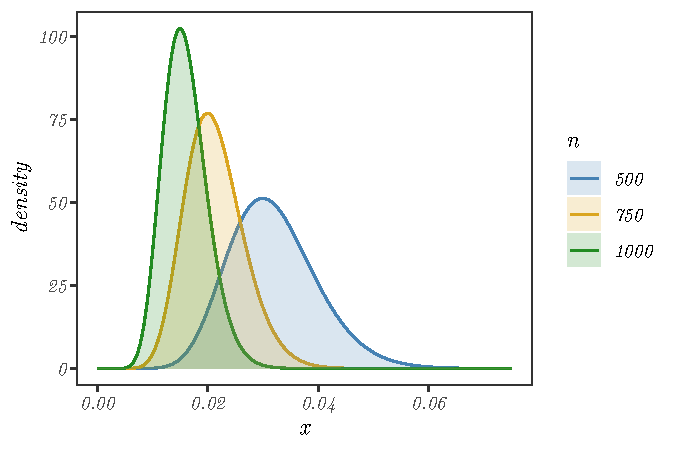
\includegraphics[width=.7\textwidth]{fig/fig-erlang-example-1.pdf}
  \caption[Probability density function of the Erlang distribution]{Probability density function $E(x, k, n+1)$ of the Erlang distribution, with $k=16$ and $n$ either 500, 750, or 1000.}
  \label{fig-erlang-example}
\end{figure}

We can now answer the second question: given $n$ and a confidence
level $\alpha$, what is the threshold value $u$ for $x_k$ such
that the probability that $x_k < u$ is equal to $\alpha$? That is,
we wish to know the value $x = u$ at which the probability
distribution has encompassed a given area of $\alpha$ (see figure~\ref{fig-alpha}).

\begin{figure}[!ht]
  \centering 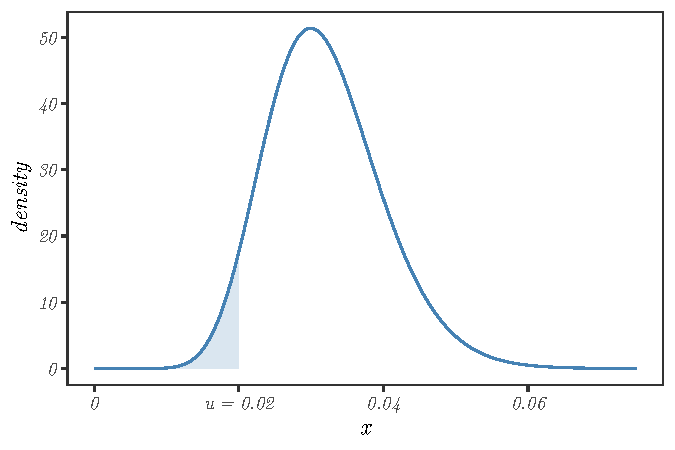
\includegraphics[width=.7\textwidth]{fig/fig-alpha-1.pdf}
  \caption[The 16th smallest value among $500$ random variates on unit interval]{The distribution of $x_{16}$, i.e., the 16th smallest value from among $n=500$ independently and uniformly drawn variates between 0 and 1. The area under the curve is shaded up to 5\% of its area. The point at which the shading stops is therefore the value $u$ for which there is only a 5\% chance of getting an even smaller $x_{16}$.}
  \label{fig-alpha}
\end{figure}

The area under
the curve of the Erlang distribution is given by its cumulative
distribution function $P(x,k,n+1)$, which is known to be
\begin{equation}\protect\hypertarget{eq-Erlang-cdf}{}{
P(x,k,n+1)
= \int_0^x E(y,k,n+1) \,\text{d}y
= \frac{1}{(k-1)!} \int_0^{(n+1)x} t^{k-1}\text{e}^{-t} \,\text{d} t .
}\label{eq-Erlang-cdf}\end{equation} The latter expression is sometimes
written as $\tilde{\gamma}(k,(n+1)x)$, where
\begin{equation}\protect\hypertarget{eq-gamma-regularized}{}{
\tilde{\gamma}(k,x)
= \frac{1}{\Gamma(k)} \int_0^x t^{k-1} \text{e}^{-t} \,\text{d}t
}\label{eq-gamma-regularized}\end{equation} is the regularized lower
incomplete gamma function. We therefore want to solve the equation
\begin{equation}\protect\hypertarget{eq-alpha}{}{
\alpha
= \int_0^u E(y,k,n+1) \,\text{d}y = P(u,k,n+1)
}\label{eq-alpha}\end{equation} for $u$.

Inverting this expression in $u$ (since the cumulative distribution
function increases monotonically in $u$, the inverse exists) leads to
the quantile function $Q(\alpha,k,n+1)$ of the Erlang distribution:
$u = Q(\alpha,k,n+1)$.
The quantile function is known to be expressible as
\begin{equation}\protect\hypertarget{eq-erlang-quantile}{}{
Q(\alpha,k,n+1)
= \frac{\tilde{\gamma}^{-1}(k,x)}{n+1} ,
}\label{eq-erlang-quantile}\end{equation} where
$\tilde{\gamma}^{-1}(k,x)$ is the inverse regularized lower incomplete
gamma function. Its particular form is of no interest to us, except for
two properties. First, it is positive for all $x$.%
%
\footnote{This stands to
reason: the quantile function of a distribution on
$x \in [0, \, \infty)$ is itself between 0 and $\infty$, and
$\tilde{\gamma}^{-1}(k,x)$ is just the quantile function of the Erlang
distribution times the positive constant $n+1$.}
%
Second, it is
independent of $n$. Instead, the entire dependence of
$Q(\alpha,k,n+1)$ on $n$ is given by the $n+1$ term in the
denominator of Equation~\ref{eq-erlang-quantile}. From this, we conclude
that $Q(\alpha,k,n+1)$ is a strictly decreasing function of $n$.

These two points lead to an important consequence. Say we compute the
threshold $u$ for a given $\alpha$ and $n$ in order to have an upper bound on a lower quantile. Now, if we were to
decrease $n$ but hold all other things equal, the threshold will
always get higher than what it was before. The threshold obtained for
higher values of $n$ may therefore serve as a conservative estimate of
the threshold for lower values: if $u$ is a threshold such that the
$k$th smallest out of $n$ uniform variates is only smaller than $u$ in
$\alpha$ of cases, then for any amount $m<n$, the chance of the
$k$th variate conforming to the same constraint (i.e., $x_k<u$) is now even smaller than $\alpha$. 

Conversely, if we were to constrain $x_k$ so that the probability of not getting a value smaller than $u$ is lower than $\beta$ (minimising a higher quantile), we find that the constraint remains true as $n$ is increased.

Armed with these results, let us see how
Equation~\ref{eq-erlang-quantile} can be used for the estimation
procedure.  
There are two problems to tackle, ultimately relating to the two aspects of a test's accuracy. First, we want to catch inadequate storers slacking on volume. In other words, we want to constrain the $x_k$ values so that we can safely say that any attacker with a stored volume below an acceptable size $n$ has a probability less than $\alpha$ to obtain such a small $x_k$ by pure chance. Construing the condition for $x_k<u$ as a test to filter honest players (just based on the size of their reserve), $1-\alpha$ expresses the \emph{sensitivity} of the test.
From the previous argument on the monotonic dependence of $\alpha$ on $n$, it is safe to use a condition that requires $x_k$ to stay below a threshold obtained for $n$. 

Second, we want to avoid situations when honest participants end up not satisfying the above constraint even though they sampled from a set larger than the required minimum. Given a target volume $m>n$, the error rate of false negatives is guaranteed to be less than $\beta$ obtained from the quantile function with parameters $m, k, \text{ and }u$. The quantity $1-\beta$ is the \emph{specificity} or \emph{precision}
of the test.



Figure~\ref{fig-ns} illustrates this
idea, for two different distributions in both the lower- and upper-end
estimation. What we want is to choose $u$ to simultaneously make sure
that dishonest players do not sneak through the system \emph{and} also that
honest players do not get excluded too often. This translates to make both $\alpha$
and $\beta$ as small as possible. 


\begin{figure}[!ht]
  \centering
  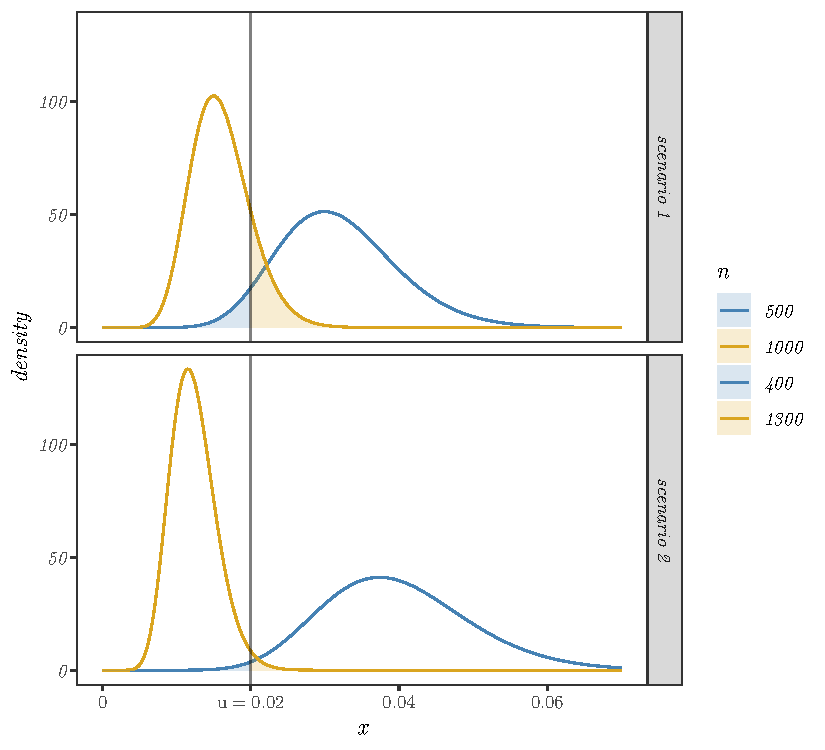
\includegraphics[width=.7\textwidth]{fig/fig-ns-1.pdf}
  \caption[Recall and precision of proof of reserve size validation]{Recall and precision of proof of reserve size validation: Any chosen $u$ will lead to different $\alpha$ and $\beta$ values, depending on $n$. Here $u$ is fixed at $0.02$. The top panel shows distributions for $x \equiv x_{16}$ with $n = 500$ (blue) and $n = 1000$ (yellow). The area left under the blue curve to the left of $u$ is equal to $\alpha$ (blue shade); the area under the yellow curve right of $u$ is equal to $\beta$ (yellow shade). If the curves overlap considerably (top), it is impossible to choose an $u$ such that $\alpha$ and $\beta$ are simultaneously small.}
  \label{fig-ns}
\end{figure}


One way to try and find the best compromise is by minimising
$\alpha + \beta$ (the \emph{accuracy} of the test) and pick the $u$ value at the optimum to be used in the proof of resources test. To this end, one
can vary $\alpha$ between 0 and 1 and, for each of its values, solve
the equation $\alpha = Q(1-\beta, k, n+1)$ (where $n$ is the larger
value, used for estimating $\beta$). This way, we get a $\beta$
value for every possible $\alpha$. Then, we can find the combination
which minimises $\alpha + \beta$, and determine the value of $u$
that leads to this optimum. As illustrated in
figure~\ref{fig-optim}, larger values of $k$ yield a trade-off curve along which
better accuracies can be achieved.

\begin{figure}[!ht]
  \centering
  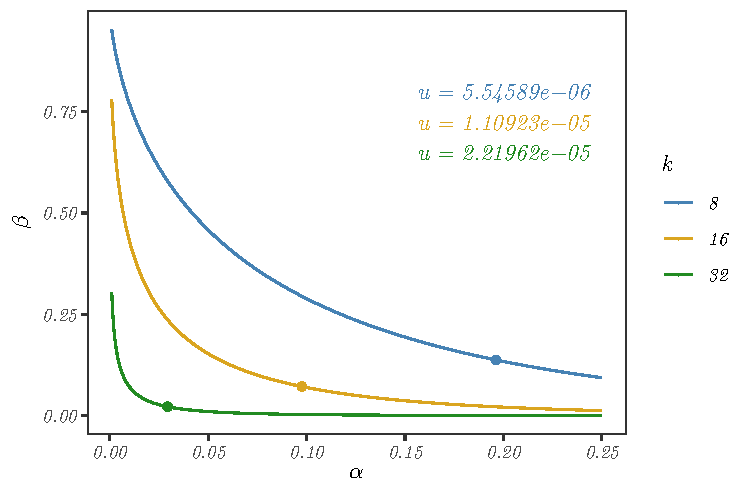
\includegraphics[width=.7\textwidth]{fig/fig-optim-1.pdf}
  \caption[Optimal accuracy of reserve size probe]{Optimal accuracy of reserve size probe By increasing $k$, one can get better optima for minimising $\alpha + \beta$. Here $n = 10^6$ for estimating $\alpha$ and $2\cdot 10^6$ for estimating $\beta$, and $k$ is either 8, 16, or 32 (colors). The values of $u$ associated with the optima are also shown.}
  \label{fig-optim}
\end{figure}



Table~\ref{tab:estim} summarizes the important numerical results in
Figure~\ref{fig-optim}.%
%
\footnote{Since the hash function used to generate random
variates does so in the range $[0, \, 2^{256}-1]$ instead of
$[0, \, 1]$, the calculated thresholds are scaled with $2^{256}$ to
show where they would fall in their actual range.}


\begin{table}[!ht]
 \centering
  \begin{tabular}{rrrrr}
  \toprule
  $k$ & $\alpha$ & $\beta$ & $u$ & $u \cdot 2^{256}$ \\
  \midrule
  8 & 0.196216 & 0.1373622 & $5.54589\cdot 10^{-6}$ & $6.421705\cdot 10^{71}$\\
  16 & 0.097612 & 0.0716570 & $1.10923\cdot 10^{-5}$ & $1.284401\cdot 10^{72}$\\
  32 & 0.029386 & 0.0219151 & $2.21962\cdot 10^{-5}$ & $2.570140\cdot 10^{72}$\\
  \bottomrule
  \end{tabular}
   \caption[Proof of density parameter calibration]{Proof of density parameter calibration. Assuming $n = 10^6$ and $m=2\cdot 10^6$ to calculate recall and precision error rates $\alpha$ and $\beta$, respectively, the cutoff value for the proof is calibrated by optimizing on acccuracy using sample sizes $8, 16, 32$.}
  \label{tab:estim}
\end{table}

\chapter{Batch utilisation}\label{sec:appendix-batch-utilisation}


When pushing content to the Swarm network, uploaders are required to
attach an attestation of storage rent prepayment to each chunk they
post. The latter is essentially a wallet registered on the postage
contract seeded with a balance from which storage rent is deduced by the
network-wide incentive system. Since this is reminiscent of buying a
batch of postage stamps and attaching one to each envelope to be posted,
the attestations are called \emph{postage stamps} and the registered
wallet a \emph{postage batch.} One can think of batches as collections
of \emph{storage slots.} The size of a batch is the number of storage
slots and is always specified as a power of 2, with the exponent
called \emph{batch depth.} Each slot can hold at most one chunk.
Putting a chunk into a slot is like issuing a postage stamp.

In practice, the attached postage stamps are digital signatures which
associate the address of a chunk with a \emph{storage slot reference.}
This in turn is composed of 1) a reference to the wallet through its
\emph{batch ID,} and 2) a \emph{within-batch index.} The fact that each
slot can hold at most one chunk ensures that batches cannot issue more
stamps than the volume registered with them. However, for an
\emph{overissuance} incident to be detectable locally by storer nodes,
the within-batch indices are arranged such that the highest $n$ bits
match the prefix of the chunk they are assigned to. These $n$ bits
define $2^n$ \emph{buckets}, the other half of the index is essentially a counter within the buckets, which is
sequentially assigned to chunks. If
the batch depth is $d$ and there
are $2^n$ buckets, then each bucket will hold a maximum of $2^{d-n}$
chunks. $k=d-n$, the log size of a bucket is called
\emph{bucket depth}. The bucket size ($2^k$) provides an exclusive upper bound to
within-bucket indices. This enforces a uniformity of stamp issuance across the $2^n$ buckets, therefore $n$ is called \emph{uniformity depth}.

Overusing a batch is now easily detected by any storer node as long as
their storage depth is shallower than the batch's uniformity depth. In
that case, each bucket of a batch is entirely within the node's reserve.
Overissuance is therefore immediately caught, since the multiple chunks 
assigned to the same slot index are seen by any node in that
neighbourhood.

When all slots are filled, we say the batch is \emph{fully utilised.} 
Although the \emph{a priori} distribution of chunks is uniform (and
therefore the expected number of chunks falling into each bucket is the
same), their stochastic assignment means that there is necessarily some variance. 
It is practically
impossible to fully fill all buckets before eventually attempting to add to one that is already full. 
We assume that the uploader is unable to
affect the address of the chunks (unencrypted fixed content) so in this scenario they are unable to
continue uploading. Because of this, one may legitimately consider the
batch to be no longer usable. The number of stamps hitherto issued by
the batch is called its \emph{effective batch size,} and its ratio to
the batch size its \emph{batch utilization rate.}

Below we explore the effect of batch parameters on their utilization
rate. With an insight into utilization rates as a function of the number
of buckets $2^n$ and the size of buckets $2^k$, we will have a way
to calibrate the expected effective batch size to be presented to users
in the context of a batch purchase user experience.

The problem of assigning chunks to storage slots is analogous with the
process of throwing marbles, one after the other, in boxes which are
initially empty. Each throw may end up in any of the boxes with equal
probability, and thus the marbles get distributed across the boxes more
or less evenly through time. However, the time will come when the boxes
start filling up. At that point, a marble may by chance end up being
thrown into a box that is already full, and thus get rejected.
Substituting chunks for marbles, buckets for boxes, and the act of
signing a stamp for throwing a marble, we recover our original scenario.
Marbles ending up in a box with equal probability corresponds to the
fact that a random chunk has equal chance of being assigned to a bucket
since the hash function has uniform distribution. Repeated rounds of
marble throwing correspond to consecutive stamping of multiple chunks of
the uploaded content; rounds constitute repeated independent trials.

Taking a particular bucket, each round of stamping is a ``success'' if
the stamp falls into the bucket, and a ``failure'' otherwise. Due to the
fact that a marble may end up in each box with equal chance, the
probability of success is $1/n$ and the probability of failure is
$1 - 1/n$. The number of stamps issued to the bucket after a given
number of rounds is described by the
\href{https://en.wikipedia.org/wiki/Negative_binomial_distribution\#Distribution_of_a_sum_of_geometrically_distributed_random_variables}{negative
binomial distribution} $\mathcal{B}(k, 1/n)$, where the first
parameter $k$ is the number of failed rounds before we stop counting,
and the second parameter is the probability of success.

The negative binomial distribution $\mathcal{B}(k, 1/n)$ is equivalent
to the sum of $k$ independent geometrically distributed variables with
parameter $1/n$. Unless $k$ is very small, the central limit theorem
ensures that this sum converges to a normal distribution. Formally, if
$\mathcal{Y}_i(1/n)$ are independent geometrically distributed
variables with parameter $1/n$, and $\mathcal{N}(\mu, \sigma^2)$ is
the normal distribution with mean $\mu$ and variance $\sigma^2$,
then for large $k$ we have
\begin{equation}\protect\hypertarget{eq-binomial-approximation}{}{
\mathcal{B}(k, 1/n) = \sum_{i=1}^k \mathcal{Y}_i(1/n) \approx \mathcal{N}(kn, kn(n-1))
}\label{eq-binomial-approximation}\end{equation} The reason for the
above form of the mean and variance in the normal distribution is as
follows: given a single geometrically distributed variable with
parameter $1/n$, its mean is $n$ and its variance is $n(n-1)$.
When adding these up over $k$ independent variables, we arrive at
$\mu = k n$ and $\sigma^2 = k n (n - 1)$ in the limiting normal
distribution.

The fit of the normal distribution with the negative binomial is robust even for
low values of $k$, as depicted in Figure~\ref{fig-normal-binomial}.

\begin{figure}
  \centering
  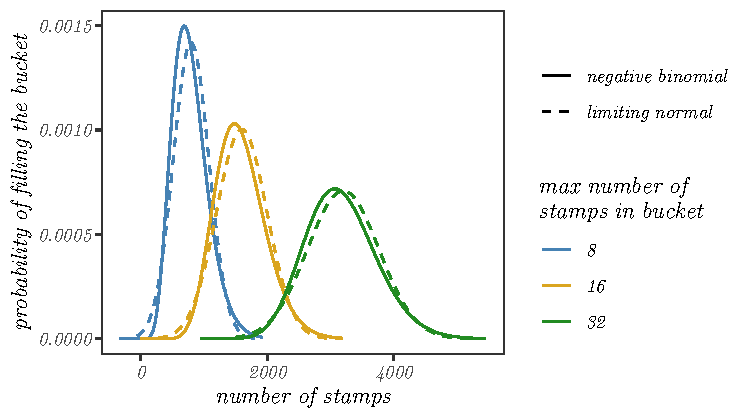
\includegraphics[width=0.7\textwidth]{fig/fig-normal-binomial-1.pdf}
  \caption[Approximating negative binomial]{\label{fig-normal-binomial}Approximating negative binomial distributions with limiting normal ones. The number of buckets $n$ is fixed at 100.}
\end{figure}

The negative binomial distribution estimates the number of rounds a
particular bucket fills up, given its size $k$ and the number of
buckets $n$. The rounds of stamping can be conceived of as parallel
independent attempts at filling up buckets. Stamps issued for failed
rounds still end up in one of the other $n - 1$ buckets, and therefore
the same probability variable counts the total stamps issued by the
batch in all buckets at the time the first one fills up. Thus, we want
to know how the \emph{minimum} of $n$ independent normal variates,
$X = \min_{i \in \{1\ldots n\}} \mathcal{N}_i(\mu, \sigma^2)$, is
distributed.

This so-called \emph{extreme value distribution} would give us the
distribution of the absolute number of total rounds needed until the
first event when one of the buckets fills up. Therefore its mean is
exactly the expected value of the number of rounds until the first
bucket-filling event. Since this is when the batch is considered
effectively used up, the mean of the distribution measures the effective
utilization of the batch. Dividing by $n$ gives the expected number of
stamps per bucket making the rate comparable across any parameter of
bucket size. Further dividing by $k$ in turn gives the \emph{expected
normalized utilization rate}, which is now comparable across all $k$
and $n$ values.

The extreme value distribution for the minimum of $n$ independent
variates drawn from the standard normal distribution (with zero mean and
unit variance) is known. It is the
\href{https://en.wikipedia.org/wiki/Gumbel_distribution}{Gumbel
distribution}, which reads
\begin{equation}\protect\hypertarget{eq-gumbel}{}{
\mathcal{G}(x; \alpha, \beta) = \frac{1}{\beta} \exp\left[
\frac{x + \alpha}{\beta} - \exp\left(\frac{x + \alpha}{\beta}\right)\right] .
}\label{eq-gumbel}\end{equation} Here $x$ is the independent variable
(in our case, the number of rounds of stamping), and $\alpha$ and
$\beta$ are the \emph{location} and \emph{scale} parameters,
respectively.\footnote{The Gumbel distribution is often given using the
  convention that one is looking for the maximum of $n$ normal
  variates, instead of their minimum. One can change between the two by
  simply flipping the sign of $x$.} They are in turn given by
\begin{equation}\protect\hypertarget{eq-loc-scale}{}{
\begin{aligned}
  \alpha &= \rho\left( 1 - \frac{1}{n} \right) ,
  \\
  \beta &= \rho\left( 1 - \frac{\text{e}^{-1}}{n} \right) - \alpha ,
\end{aligned}
}\label{eq-loc-scale}\end{equation} where
$\text{e}^{-1} = \exp(-1) \approx 0.368$, $n$ is the number of
normal variates whose minimum we are looking for, and $\rho(x)$ is the
quantile function of the normal distribution (or the inverse of the
\href{https://en.wikipedia.org/wiki/Error_function}{error function}).
The mean, standard deviation, and quantile function of the Gumbel
distribution are
\begin{equation}\protect\hypertarget{eq-mean-var-quantile}{}{
\begin{aligned}
  \mathbb{E}(\mathcal{G}) &= \alpha + \gamma \beta ,
  \\
  \mathbb{S}(\mathcal{G}) &= \beta \, \frac{\pi}{\sqrt{6}} ,
  \\
  Q(p; \mathcal{G}) &= \beta \, \log(-\log(1 - p)) - \alpha ,
\end{aligned}
}\label{eq-mean-var-quantile}\end{equation} where
$\gamma \approx 0.5772$ is the Euler--Mascheroni constant, and
$0 < p < 1$ in $Q(p; \mathcal{G})$ is a probability quantile.

The normal distribution whose variates' minimum values we are looking
for is not standard, but instead has mean $\mu = k n$ (instead of
zero), and variance $\sigma^2 = k n (n-1)$ (instead of one).
Therefore, the Gumbel distribution needs to be appropriately rescaled.
Denoting this scaled probability distribution by $\mathcal{X}$, we
have \begin{equation}\protect\hypertarget{eq-gumbel-scaled}{}{
  \mathcal{X}(x; \mu, \sigma, \alpha, \beta) =
  \frac{1}{\sigma}\mathcal{G}\left(\frac{x - \mu}{\sigma}; \alpha, \beta\right)
}\label{eq-gumbel-scaled}\end{equation} (the overall factor of
$1 / \sigma$ restores the proper normalization of the scaled
function). Consequently, the mean, standard deviation, and quantile
function should also be rescaled:
\begin{equation}\protect\hypertarget{eq-mean-var-quantile-scaled}{}{
\begin{aligned}
  \mathbb{E}(\mathcal{X}) &= \mu - \sigma (\alpha+\gamma\beta) = kn-\sqrt{kn(n-1)}
  \left[(1-\gamma) \rho\left( 1 - \frac{1}{n} \right) + \gamma \rho\left( 1 -
  \frac{\text{e}^{-1}}{n} \right) \right] , 
  \\
  \mathbb{S}(\mathcal{X}) &=\sigma \beta \frac{\pi}{\sqrt{6}} =
  \sqrt{ k n (n-1)} \left[ \rho\left( 1 - \frac{\text{e}^{-1}}{n} \right) -
  \rho\left( 1 - \frac{1}{n} \right) \right] \frac{\pi}{\sqrt{6}} ,
  \\
  Q(p;\mathcal{X})&= \mu-\sigma\left[\alpha-\beta \,
  \log(-\log(1-p))\right] \\ &= kn-\sqrt{ k n (n-1)}\left[\rho\left( 1 -
  \frac{1}{n} \right)-\rho\left( 1 - \frac{\text{e}^{-1}}{n} \right) 
  \log\left(-\log(1-p)\right)\right] .
\end{aligned}
}\label{eq-mean-var-quantile-scaled}\end{equation} Normalizing the mean
and the quantile function by the product $kn$:
\begin{equation}\protect\hypertarget{eq-mean-quant-div}{}{
\begin{aligned}
  \frac{\mathbb{E}(\mathcal{X})}{k n} &= 1 - \sqrt{\frac{(n-1)}{kn}} \left[ (1-\gamma)
  \rho\left( 1 - \frac{1}{n} \right) + \gamma \rho\left( 1 - \frac{\text{e}^{-1}}{n}
  \right) \right] ,
  \\
  \frac{Q(p; \mathcal{X})}{kn} &= 1 - \sqrt{\frac{(n-1)}{kn}}
  \left[\rho\left( 1 - \frac{1}{n} \right)-\rho\left( 1 - \frac{\text{e}^{-1}}{n}
  \right)  \log\left(-\log(1-p)\right)\right] .
\end{aligned}
}\label{eq-mean-quant-div}\end{equation} Taking into account that $k$
and $n$ must both be powers of two, we can write $k = 2^{\kappa}$
and $n = 2^{\nu}$, where $\kappa$ and $\nu$ are positive integers.
We then have \begin{equation}\protect\hypertarget{eq-mean-div-simp}{}{
  \frac{\mathbb{E}(\mathcal{X})}{k n} =
  \frac{\mathbb{E}(\mathcal{X})}{2^{\kappa + \nu}} =
  1 - \sqrt{\frac{2^\nu-1}{2^{\kappa+\nu}}}\left[ (1-\gamma) \rho\left( 1 -
  \frac{1}{2^{\nu}} \right) + \gamma \rho\left( 1 - \frac{\text{e}^{-1}}{2^{\nu}}
  \right) \right] .
}\label{eq-mean-div-simp}\end{equation}

In order to explore this solution, we consider the average expected
utilization rate as a function of uniformity depth, for various log bucket
sizes (see Figure~\ref{fig-mean}). As long as bucket size is around $2^8$ or greater,
the dependence of the utilization rate on $n$ is milder and milder, and at $2^{16}$, it is virtually a flat line at $100\%$.
In general, we see that for the same bucket size, the miss rate
(one minus the utilization rate) increases with the number of buckets. Using
small bucket sizes (up to $2^{10}$), we get unacceptably high miss
rates even with few buckets.%
%
\footnote{Note that for low $k$ but high
  $n$, the solution is unreliable, predicting a negative number of
  stamps per bucket. The prediction will generally not work well if
  $k$ is too small, because the normal approximation to the negative
  binomial distribution starts to break down.}
%  
On the other hand, for
larger bucket sizes (over $2^{10}$), the miss rate is contained at a
tolerable $<10\%$ (on the right in Figure~\ref{fig-mean}).

On the right, we plot the miss rate on a logarithmic scale as a function of log bucket size, for various numbers of buckets. We
find that doubling the batch size 6 times decreases the miss rate
tenfold, regardless the actual size or the number of buckets. In fact,
as the close parallel lines show (on the right in Figure~\ref{fig-mean}), there is no interaction:
going from one bucket to a billion increases the miss rate
only by tenfold, independently of bucket size.


\begin{figure}[!ht]
  \centering
  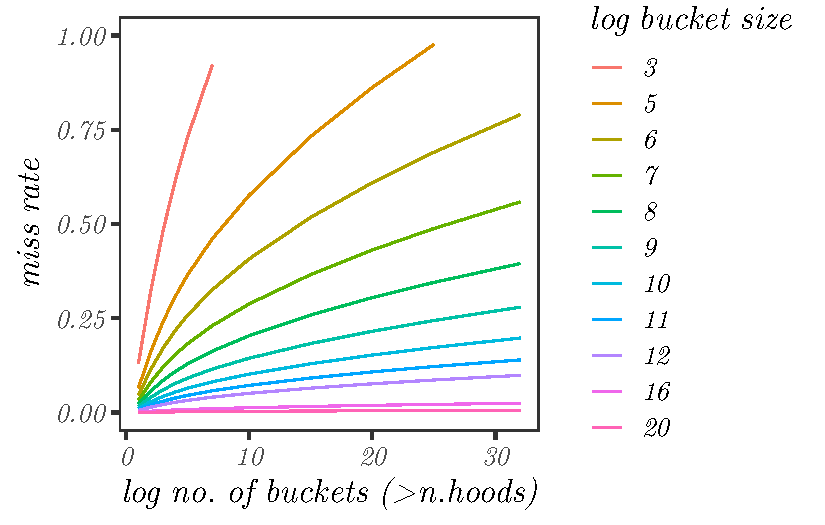
\includegraphics[width=0.49\textwidth]{fig/fig-mean-1.pdf} 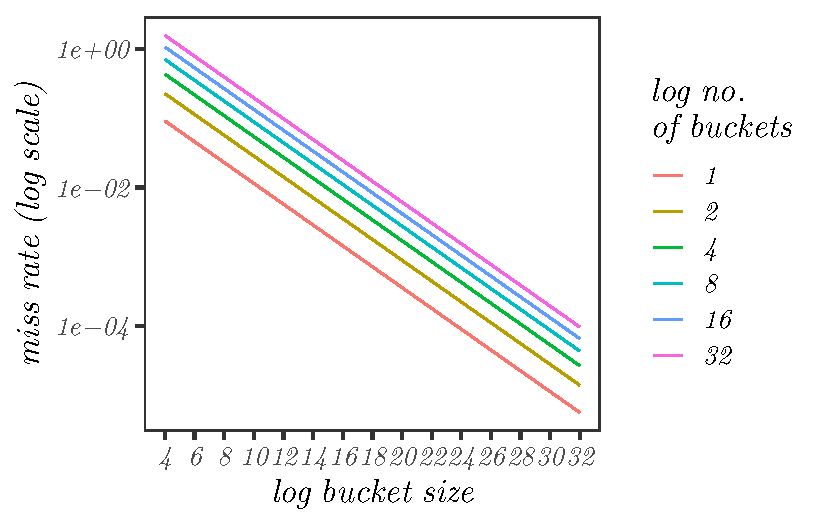
\includegraphics[width=0.49\textwidth]{fig/fig-mean-2.pdf}
  \caption[Expected miss rate, for various parameters.]{\label{fig-mean}Expected miss rate, for various parameters. Left: miss rate against the number of buckets. Right: miss rate against bucket size.}
\end{figure}


\begin{figure}[!ht]
  \centering
  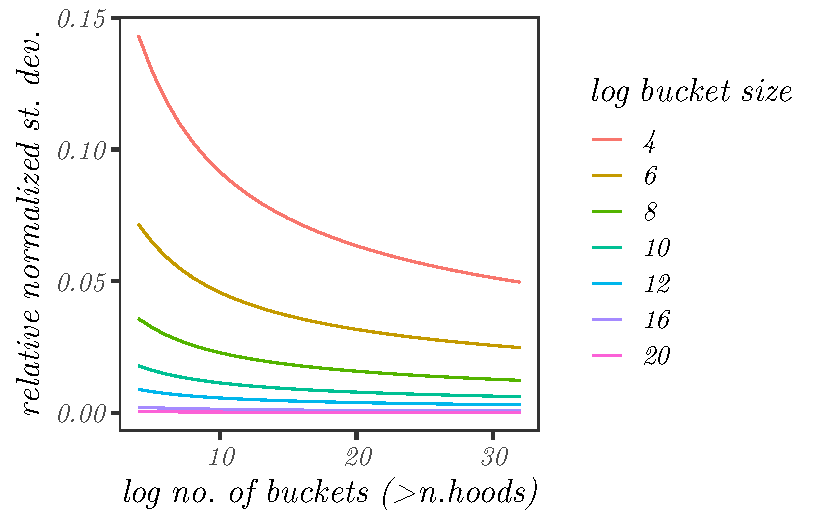
\includegraphics[width=0.49\textwidth]{fig/fig-sd-1.pdf} 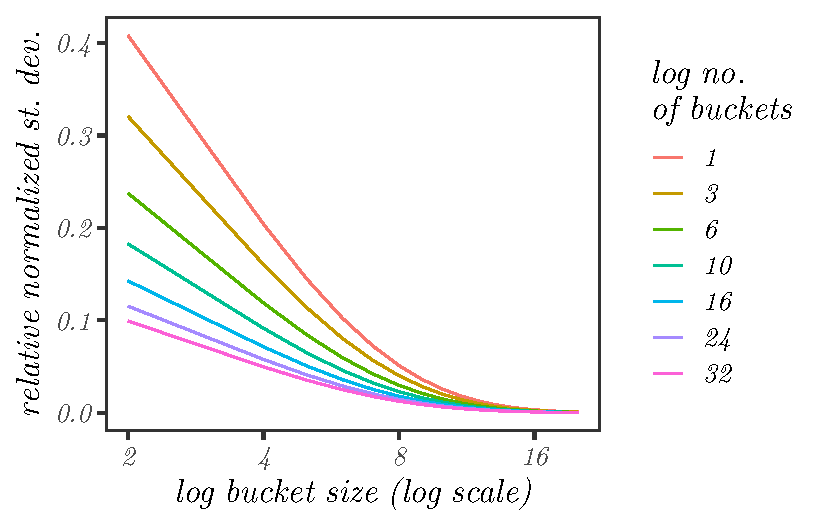
\includegraphics[width=0.49\textwidth]{fig/fig-sd-2.pdf}
  \caption[Normalized standard deviation of utilization rate]{\label{fig-sd}Normalized standard deviation of utilization rate, for various parameters. Left: relative standard deviation against the number of buckets. Right: relative standard deviation against bucket size.}
\end{figure}




Looking at relative standard deviation of the distribution for various values of $k$ and $n$ (see Figure~\ref{fig-sd}), we find not much variance whenever $k$ and $n$ are large. Nevertheless, for the sake of correctness, we check the quantile function of our extreme value distribution (see Figures~\ref{fig-qua} and \ref{fig-q}).

\begin{figure}[!ht]
  \centering
  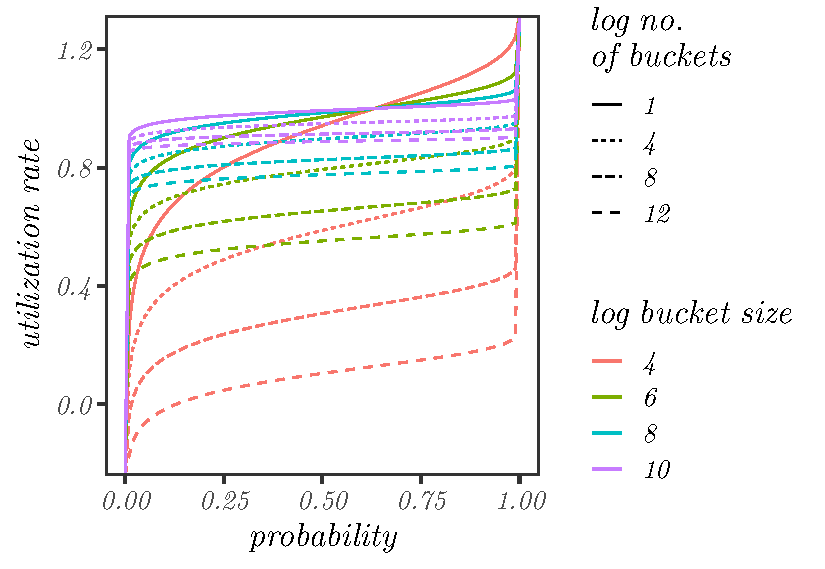
\includegraphics[width=0.49\textwidth]{fig/fig-qua-1.pdf} 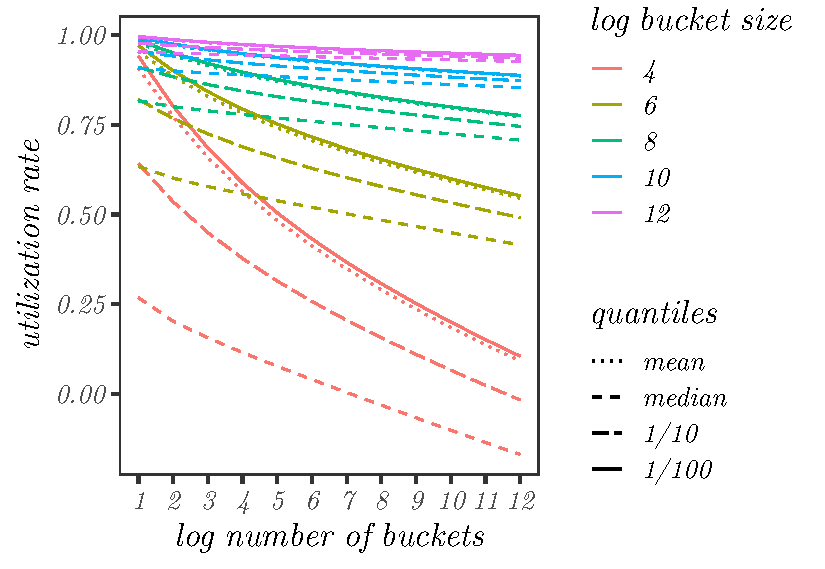
\includegraphics[width=0.49\textwidth]{fig/fig-qua-2.pdf}
  \caption[Quantiles of the utilization rate]{\label{fig-qua}Quantiles of the utilization rate, for
various parameters. Left: the quantile function of the utilization
rate. Right: mean, median, 10\%, and 1\% percentiles of utilization against the number of buckets.}
\end{figure}

\begin{figure}[!ht]
  \centering
  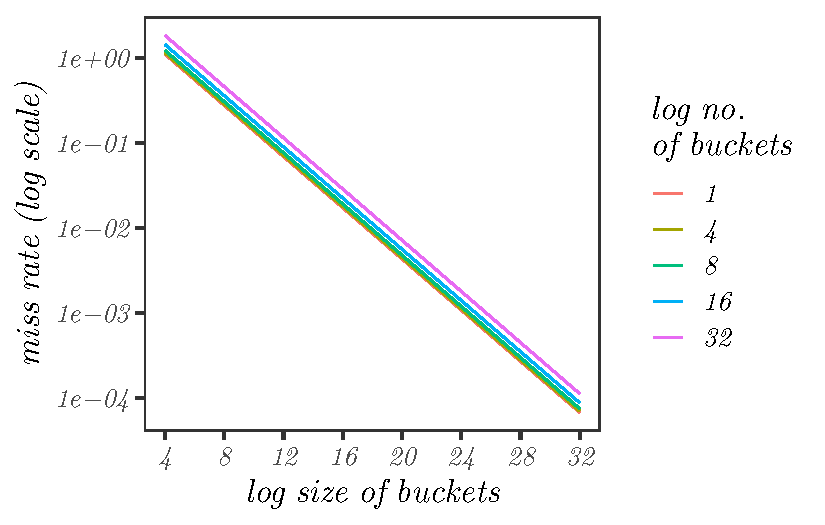
\includegraphics[width=0.49\textwidth]{fig/fig-q-1.pdf} 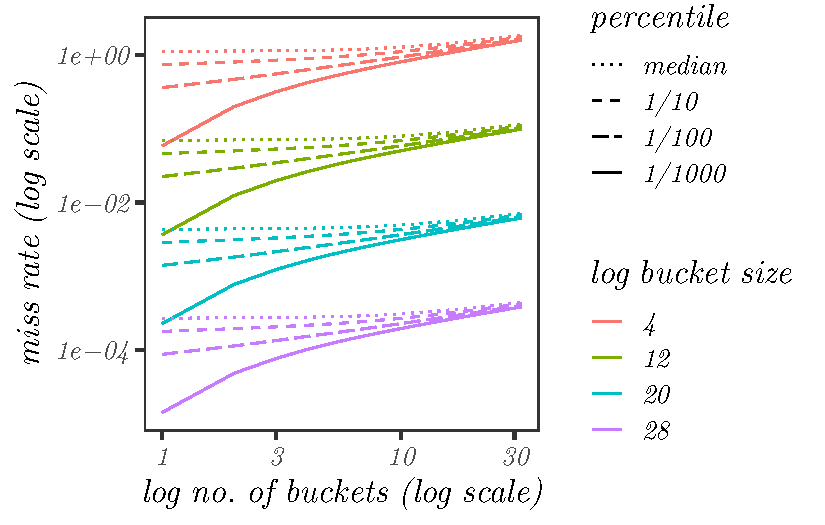
\includegraphics[width=0.49\textwidth]{fig/fig-q-2.pdf}
  \caption[Quantiles of the miss rate]{Quantiles of the miss rate for various parameters. Left: one-in-a-thousand quantile for miss rate against bucket size. Right: miss rate in terms of percentiles, against number of buckets.}
\label{fig-q}
\end{figure}

 
Eventually, we aim to use the information on utilization rates to
protect the user from being surprised at the effective utilization of
their postage batch. To this end, we apply the volume calibration using
a reasonable worst-case scenario, i.e., define the effective utilization
rate as the one-in-a-thousand low-tail quantile of the utilization rate.
To obtain the ``effective'' volumes, we simply multiply the theoretical
purchased volume (given by $2^d$ where $d$ is the batch depth) by
the effective utilization rate.


Finally, in table~\ref{tab:batch-utilisation}, we provide these volume calibrations for $2^{12}$ and
$2^{16}$ buckets and log bucket sizes ranging from $4$ to $25$.
Above this bucket size the required quantile already shows a miss rate
below $0.1\%$. That is, there is only a one-in-a-thousand chance that
the difference between the effectively utilized volume and the
theoretically purchased one exceeds one tenth of a percent which we
consider insignificant enough to justify no calibration on the
theoretical volume.

\newpage

\begin{longtable}{rrrrrr}\toprule
\multicolumn{1}{c}{log2 no.}& 
\multicolumn{1}{c}{log2 size} & 
\multicolumn{1}{c}{log2 no.}&
\multicolumn{1}{c}{utilisation}&
\multicolumn{1}{c}{theoretical}&
\multicolumn{1}{c}{effective}\\
\multicolumn{1}{c}{of buckets}&
\multicolumn{1}{c}{of buckets}&
\multicolumn{1}{c}{of chunks}&
\multicolumn{1}{c}{rate}&
\multicolumn{1}{c}{volume}&
\multicolumn{1}{c}{volume}\\
\midrule
12 & 4 & 16 & 0.00000 & 268.44 MB & 0.00 B \\
12 & 5 & 17 & 0.06747 & 536.87 MB & 36.22 MB \\
12 & 6 & 18 & 0.34060 & 1.07 GB & 365.72 MB \\
12 & 7 & 19 & 0.53374 & 2.15 GB & 1.15 GB \\
12 & 8 & 20 & 0.67030 & 4.29 GB & 2.88 GB \\
12 & 9 & 21 & 0.76687 & 8.59 GB & 6.59 GB \\
12 & 10 & 22 & 0.83515 & 17.18 GB & 14.35 GB \\
12 & 11 & 23 & 0.88343 & 34.36 GB & 30.35 GB \\
12 & 12 & 24 & 0.91758 & 68.72 GB & 63.06 GB \\
12 & 13 & 25 & 0.94172 & 137.44 GB & 129.43 GB \\
12 & 14 & 26 & 0.95879 & 274.88 GB & 263.55 GB \\
12 & 15 & 27 & 0.97086 & 549.76 GB & 533.74 GB \\
12 & 16 & 28 & 0.97939 & 1.10 TB & 1.08 TB \\
12 & 17 & 29 & 0.98543 & 2.20 TB & 2.17 TB \\
12 & 18 & 30 & 0.98970 & 4.40 TB & 4.35 TB \\
12 & 19 & 31 & 0.99271 & 8.80 TB & 8.73 TB \\
12 & 20 & 32 & 0.99485 & 17.59 TB & 17.50 TB \\
12 & 21 & 33 & 0.99636 & 35.18 TB & 35.06 TB \\
12 & 22 & 34 & 0.99742 & 70.37 TB & 70.19 TB \\
12 & 23 & 35 & 0.99818 & 140.74 TB & 140.48 TB \\
12 & 24 & 36 & 0.99871 & 281.47 TB & 281.11 TB \\
12 & 25 & 37 & 0.99909 & 562.95 TB & 562.44 TB \\
16 & 4 & 20 & 0.00000 & 4.29 GB & 0.00 B \\
16 & 5 & 21 & 0.00000 & 8.59 GB & 0.00 B \\
16 & 6 & 22 & 0.28669 & 17.18 GB & 4.93 GB \\
16 & 7 & 23 & 0.49561 & 34.36 GB & 17.03 GB \\
16 & 8 & 24 & 0.64334 & 68.72 GB & 44.21 GB \\
16 & 9 & 25 & 0.74781 & 137.44 GB & 102.78 GB \\
16 & 10 & 26 & 0.82167 & 274.88 GB & 225.86 GB \\
16 & 11 & 27 & 0.87390 & 549.76 GB & 480.43 GB \\
16 & 12 & 28 & 0.91084 & 1.10 TB & 1.00 TB \\
16 & 13 & 29 & 0.93695 & 2.20 TB & 2.06 TB \\
16 & 14 & 30 & 0.95542 & 4.40 TB & 4.20 TB \\
16 & 15 & 31 & 0.96848 & 8.80 TB & 8.52 TB \\
16 & 16 & 32 & 0.97771 & 17.59 TB & 17.20 TB \\
16 & 17 & 33 & 0.98424 & 35.18 TB & 34.63 TB \\
16 & 18 & 34 & 0.98885 & 70.37 TB & 69.58 TB \\
16 & 19 & 35 & 0.99212 & 140.74 TB & 139.63 TB \\
16 & 20 & 36 & 0.99443 & 281.47 TB & 279.91 TB \\
16 & 21 & 37 & 0.99606 & 562.95 TB & 560.73 TB \\
16 & 22 & 38 & 0.99721 & 1.13 PB & 1.12 PB \\
16 & 23 & 39 & 0.99803 & 2.25 PB & 2.25 PB \\
16 & 24 & 40 & 0.99861 & 4.50 PB & 4.50 PB \\
16 & 25 & 41 & 0.99901 & 9.01 PB & 9.00 PB \\
\bottomrule
\caption{Theoretical and effective volumes of postage batches}
\label{tab:batch-utilisation}
\end{longtable}


\end{document}

